\chapter{Modelado de sistemas dinámicos}
Warning: Section in progress

\section{State-space systems}
We will focus on systems that can be described by quantifiable characteristics or states, e.g., temperature, velocity or voltage. These states might change over time. One might interact with a system via a quantifiable input, and one might measure some information from the states of the system via a quantifiable output.

Let us define $x(t)\in\mathbb{R}^n$, $y(t)\in\mathbb{R}^m$ and $u(t)\in\mathbb{R}^k$ as the stacked (signal) vector of states, the output, and the input of a system $\Sigma$ respectively. In particular, we will describe them as continuous signals over time, e.g., $x :[0,\infty) \to \mathbb{R}^n$. 

The system $\Sigma$ is a model that predicts the value of the states and the output over time. This prediction incorporates the impact of the input on the states and the output. We utilize differential equations as a tool to predict the evolution of the states of the system $\Sigma$ over time as follows
\begin{equation}
	\Sigma := \begin{cases}
		\dot x(t) =& f(x(t),u(t)) \\ y(t) =& g(x(t),u(t))
	\end{cases}, 
\label{eq: sigma}
\end{equation}
where $\dot x := \frac{\mathrm{d}}{\mathrm{dt}}(x(t))$ is the short notation for total derivative with respect to time, and $f: \mathbb{R}^n \times \mathbb{R}^k \to \mathbb{R}^n$ and $g: \mathbb{R}^n \times \mathbb{R}^k \to \mathbb{R}^m$ are functions.

We can represent the system $\Sigma$ as a block with input/output ports as in figure \ref{fig: sigma}.

\begin{figure}[!h]
\centering
\begin{tikzpicture}[auto, node distance=2cm,>=latex']
	\node [input, name=input] {};
	\node [block, right of=input] (system) {$\Sigma$};
	\node [output, right of=system] (output) {};
	\draw [draw,->] (input) -- node {$u(t)$} (system);
	\draw [->] (system) -- node [name=y] {$y(t)$}(output);
\end{tikzpicture}
	\caption{Input/output block diagram of system $\Sigma$.}
	\label{fig: sigma}
\end{figure}

\section{Ejemplos}
\subsection{Inverted pendulum}

We are going to derive $f$ and $g$ for the inverted pendulum.

First, we derive the equations of motion of the mass in the inverted pendulum system in figure \ref{fig: invpen} as a first step to figure out the system's functions $f$ and $g$. Consider that we can interact with the system with a torque $T$ applied on the base, the mass is under a friction force proportional to its speed, and we can only measure the angle $\theta$ from the system.

\begin{figure}[!h]
\centering
	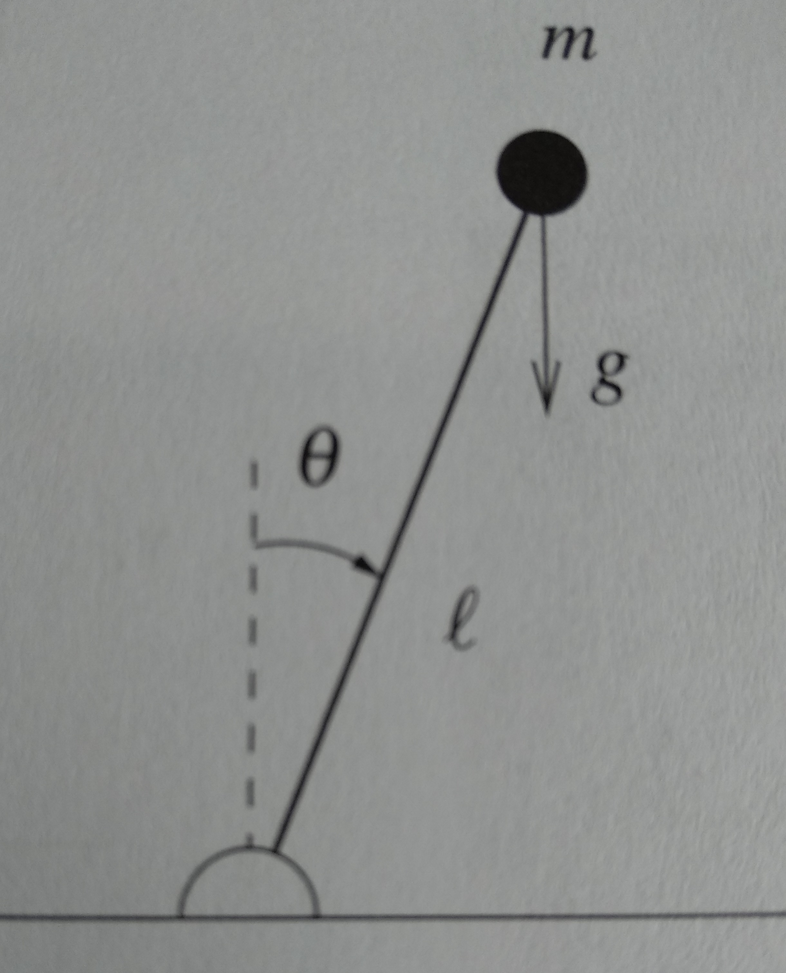
\includegraphics[scale=0.1]{./invpen.png}
	\caption{Inverted pendulum}
	\label{fig: invpen}
\end{figure}


We choose the angle $\theta$ with respect to the vertical to derive the dynamics of the inverted pendulum. Define $m, l, g,$ and $I\in\mathbb{R}$ as the mass, pendulum's lenght, gravity acceleration and inertia moment respectively. In particular, we have that $I = ml^2$, and we will exploit that $I \ddot\theta = \text{sum of torques}$. We have to consider three torques; namely: 1. Torque $T$ applied by us; 2. Torque $-b\dot\theta$ applied by the friction; 3. Torque $mgl \sin\theta$ applied by the gravitational forces, i.e., $mg$ is the force on the mass, times $\sin\theta$ since the force only applies perpendicular to the bar, and times $l$ to compute the resultant torque. Therefore the dynamics of the inverted pendulum are given by
\begin{equation}
\ddot\theta = \frac{1}{ml^2}\left(mgl\sin{\theta}-b\dot\theta + T\right).
	\label{eq: dyn}
\end{equation}

It looks reasonable to choose $\theta$ as one of our states to construct $x(t)$. In fact, since we have derived a second-order system, we will need $\dot\theta$ as a second state since we have the differential equation for its derivative $\ddot\theta$. Thus, let us define the state vector
\begin{equation}
x := \begin{bmatrix}\theta \\ \dot\theta \end{bmatrix},
\end{equation}
and since the torque $T$ is how we interact with the system, we choose the input $u(t) = T(t)$.

Now we are ready to construct the functions $f$ and $g$ in (\ref{eq: sigma}) for the inverted pendulum. In particular, we know that $f$ and $g$ only accepts as inputs/arguments the state space vector $x$ and the input $u$. On the left side of (\ref{eq: sigma}) we have the time derivative of $x(t)$, therefore
\begin{equation}
	\frac{\mathrm{d}}{\mathrm{dt}}\left(\begin{bmatrix}\theta \\ \dot\theta \end{bmatrix}\right) = f(x(t), u(t)) = \begin{bmatrix}f_1(x(t), u(t)) \\ f_2(x(t), u(t))\end{bmatrix}, \label{eq: fn}
\end{equation}
where $f_1 = \dot\theta$. Note that for the first row in (\ref{eq: fn}), on the left we have $\frac{\mathrm{d}}{\mathrm{dt}}\theta$, and on the right $f_1 = \dot\theta$ because $\dot\theta$ is actually a state, roughly speaking we can say that $\dot\theta(t) \in x(t)$. Unfortunatelly, we cannot say that $f_2 = \ddot\theta(t)$ because (roughly speaking) $\ddot\theta(t) \notin x(t)$. Nevertheless, we have that $f_2$ is given by the differential equation (\ref{eq: dyn}). Then, let me write explicitly $f$ as follows
\begin{equation}
	\frac{\mathrm{d}}{\mathrm{dt}}\left(\begin{bmatrix}\theta \\ \dot\theta \end{bmatrix}\right) =  f(x(t), u(t)) = \begin{bmatrix} \dot\theta \\ \frac{1}{ml^2}\left(mgl\sin{\theta}-b\dot\theta + T\right) \end{bmatrix}, \label{eq: f}
\end{equation}

The calculation of $g$ is more straightforward. We have established that we can only measure the angle, therefore $y(t) = \theta(t)$, i.e., 
\begin{equation}
g(x(t),u(t)) =  \theta(t).
	\label{eq: g}
\end{equation}

A Python simulation of this dynamics can be found at \url{https://github.com/noether/aut_course}.

\subsection{El oscilador de Van der Pol}
Se trata de un oscilador, propuesto por primera vez por Balthasar Van der Pol, cuando trabajaba en Philips, para explicar las oscilaciones observadas en tubos de vacío. Podemos obtener la ecuación del oscilador, empleando el circuito de la figura \ref{fig:vdp}
\begin{figure}
\centering
\begin{circuitikz}[american, scale = 0.6]\draw
(0,-4)to[short]
(4,-4)to[short,,i^<= $i_C$]
(5,-4)to[short,i=$i_N$]
(6,-4)to[short](10,-4)
(0,-7.5)to[C = C](0,-4)
(5,-4) to[L = L, i>^= $i_L$,*-* ](5,-7.5)
(10,-4) to[generic=NL,  i= $i_N \equiv h(v)$](10,-7.5) 
(0,-7.5)to[short](10,-7.5)
;
\end{circuitikz}  
\label{fig:vdp}
\caption{Circuito eléctrico no lineal}
\end{figure}

Donde el elemento no lineal NL, presenta una relación entre voltaje e intensidad caracterizada por la función $h(v)$.

El voltaje $v$ en los tres componentes del circuito debe ser igual; además,
\begin{align}
v = L \frac{di_L}{dt}\\
i_C = C\frac{dv}{dt}
\end{align}
Si aplicamos la primera ley de Kirchohff al nodo superior del circuito,
\begin{align}
i_C+i_L+i_N = 0\\
C\frac{dv}{dt}+\frac{1}{L}\int_{-\infty}^{t}v(s)ds +h(v)=0\label{eq:vdp}
\end{align}
Si derivamos \ref{eq:vdp} con respecto al tiempo, dividimos por $C$ y reordenamos,
\begin{equation}\label{eq:vdp2}
\frac{d^2v}{dt^2}  + \frac{1}{C}\frac{dh(v)}{dv}\frac{dv}{dt} + \frac{1}{LC}\cdot v= 0
\end{equation}
Se trata de un caso particular de la ecuación de Liénard,
\begin{equation}
\ddot{v} +f(v)\dot{v}+g(v) = 0
\end{equation}
Si definimos ahora, $h(v)$,
\begin{align}
h(v) = m(\frac{1}{3}v^3-1)\\
\frac{dh}{dv} = m(v^2-1)
\end{align}
y sustituyendo en \ref{eq:vdp2},
\begin{equation}
\ddot{v} +m\frac{1}{C}(v^2-1)\dot{v}+\frac{1}{LC}v = 0
\end{equation}

Podemos representarla finalmente en variables de estado, tomando $x_1=v$ y $x_2=\dot{v}$,
\begin{align}
\dot{x}_1 &= x_2\\
\dot{x}_2 &= -\frac{1}{LC}x_1 - m\frac{1}{C}(x_1^2-1)x_2 \label{eq:vdpst2}
\end{align}
Podemos ahora hacer un primer análisis cualitativo. El primer término a la derecha del igual en  la ecuación \ref{eq:vdpst2} representa una fuerza recuperadora proporcional al desplazamiento, el segundo término, crecerá con la velocidad para $x_1 < 1$, alejando así al sistema del origen  y representará un término disipativo para $x_1 > 1$ acercándolo por tanto de nuevo al origen. Es por tanto esperable, que se alcance
algún tipo de situación de equilibrio. Más adelante definiremos esta situación rigurosamente como un ciclo límite. 
\subsection{Un vehículo de cuatro ruedas. }
La figura \ref{fig:vehir} muestra un esquema de un vehículo terrestre de cuatro ruedas, visto desde arriba. Si consideramos que se mueve en el plano $x,y$, y que su velocidad instántanea $\vec{V}$ está siempre orientada en la dirección de avance del vehículo $\psi$ --asumimos que no derrapa, ni se mueve lateralmente--, podemos entonces definir la velocidad, en el sistema de referencia $x,y$ como,
\begin{align}
\dot{x} = V_x(t) = V\cos(\psi(t))\\
\dot{y} = V_y(t) = V\sin(\psi(t))\\
\end{align}

\begin{figure}
\centering

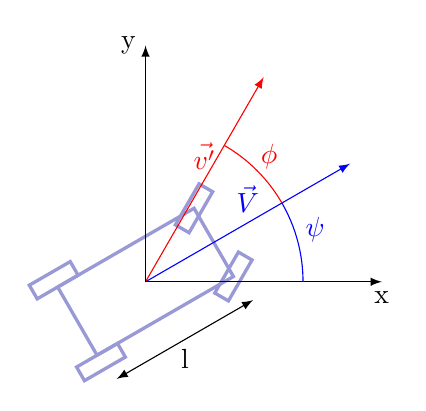
\begin{tikzpicture}
\draw(0,0)[rotate around={30:(0,0)},very thick,draw = blue!60!black!40]rectangle(2,1);
\draw(-0.3,-0.2)[rotate around={30:(0,0)},very thick,draw = blue!60!black!40]rectangle(0.3,0.0);
\draw(-0.3,1)[rotate around={30:(0,0)},very thick,draw = blue!60!black!40]rectangle(0.3,1.2);
\draw({2*cos(30)-0.3},{2*sin(30)-0.1})[rotate around={60:({2*cos(30)},{2*sin(30)})},very thick,draw = blue!60!black!40]rectangle({2*cos(30)+0.3},{2*sin(30)+0.1});
\draw({2*cos(30)-sin(30)-0.3},{2*sin(30)+cos(30)-0.1})[rotate around={60:({2*cos(30)-sin(30)},{2*sin(30)+cos(30)})},very thick,draw = blue!60!black!40]rectangle({2*cos(30)-sin(30)+0.3},{2*sin(30)+cos(30)+0.1});
\draw[blue]({cos(30)-0.5*sin(30)},{sin(30)+0.5*cos(30)})--node[above]{$\vec{V}$}({4*cos(30)-0.5*sin(30)},{4*sin(30)+0.5*cos(30)})[-latex];
\draw[red]({cos(30)-0.5*sin(30)},{sin(30)+0.5*cos(30)})--node[above]{$\vec{v'}$}({cos(30)-0.5*sin(30)+3*cos(60},{sin(30)+0.5*cos(30)+3*sin(60})[-latex];

\draw({cos(30)-0.5*sin(30)},{sin(30)+0.5*cos(30)})--({3+cos(30)-0.5*sin(30)},{sin(30)+0.5*cos(30)})[-latex]node[anchor=north]{x};
\draw({cos(30)-0.5*sin(30)},{sin(30)+0.5*cos(30)})--({cos(30)-0.5*sin(30)},{3+sin(30)+0.5*cos(30)})[-latex]node[anchor=east]{y};

\draw[blue]({2+cos(30)-0.5*sin(30)},{sin(30)+0.5*cos(30)})arc(0:30:2);
\draw[red]({3*cos(30)-0.5*sin(30)},{3*sin(30)+0.5*cos(30)})arc(30:60:2);
\draw[blue]({3.2*cos(30)},{3.2*sin(30)}) node[]{$\psi$};
\draw[red]({3.4*cos(50)},{3.3*sin(50)}) node[]{$\phi$};
\draw[latex-latex](0.25,-0.3)--node[below]{l}({2*cos(30)+0.25},{2*sin(30)-0.3});
\end{tikzpicture}
\label{fig:vehir}
\caption{Esquema de un vehículo terrestre de 4 ruedas}
\end{figure}

Además el vehículo girará, siempre que las ruedas delanteras no estén alineadas con las ruedas traseras, cambiando así su dirección de avance . Podemos relacionar la velocidad de giro del vehículo $\dot{\psi}$ con el ángulo de orientación de las ruedas delanteras $\phi$, y la velocidad a la que avanzan $\vec{v'}$.  podemos obtener las componetes de dicha velocidad en ejes cuerpo (paralela y perpendicular a la dirección de avance del vehículo),

\begin{align}
v_{P} = v'\cos(\phi(t))\\
v_{T} = v'\sin(\phi(t))
\end{align} 

Pero la rueda esta unida al vehículo así que su velocidad en la direccíon de avance debe ser la misma que la del vehículo: $v_P \equiv V$.  A partir de esta relación podemos obtener la velocidad tangencial de las ruedas como,
\begin{equation}
v_T = V\frac{\sin(\phi)}{\cos(\phi)} = V\tan(\phi)
\end{equation}

Si tomamos como centro de giro del vehículo el centro de su eje trasero, y la batalla (distancia entre ejes) es $l$, obtenemos una expresión para su velocidad de giro,
\begin{equation}
\dot{\psi} = \frac{V}{l}\tan(\phi)
\end{equation}

En resumen, podemos describir el sistema mediante tres ecuaciones de estado $x_1 \equiv x, x_2\equiv	y, x_3 \equiv \psi$:
\begin{align}
\dot{x}_1 =  V\cos(x_3)\\  
\dot{x}_2 =  V\sin(x_3)\\
\dot{x}_3 = \frac{V}{l}\tan(\phi)
\end{align}

Si consideramos $V=cte$, la única entrada al sistema sería el ángulo de giro de las ruedas $u(t) = \phi(t)$, controlando su valor, podemos hacer girar al vehículo en la dirección deseada. 

\section{Simulations / Numerical solutions}
We can still calculate numerical solutions (also known as simulations) for $\Sigma$ given a starting point $x(0)$. The \emph{Euler integration} is an easy numerical method that can give us some information about $\Sigma$. The following algorithm is what you can use in your Python/Matlab simulations
\begin{algo}
	\begin{enumerate}
		\item Set step time $\Delta T$
		\item Set $x = x(0)$
		\item Set $y = g(x,u)$
		\item Log $x$ and $y$, so you can plot them later
		\item Set $t = 0$
		\item Set final time $T^*$
		\item While $t \leq T^*$ then:
			\begin{enumerate}
				\item Set $x_{\text{new}} = x_{\text{old}} + f(x_{\text{old}},u)\Delta T$
				\item Set $y_{\text{new}} = g(x_{\text{new}},u)$
				\item Draw $x$
				\item Log $x$ and $y$, so you can plot them later
				\item Set $t = t + \Delta t$
			\end{enumerate}
		\item Plot the log for the elements of $x$ and $y$ over time $t$
	\end{enumerate}
\end{algo}
This algorithm performs okei when $\Delta T$ is sufficiently small. How small? It always depends on the system $\Sigma$, in particular, of $f$. Check \url{https://en.wikipedia.org/wiki/Euler_method} for more details, and of course, for more accurate methods. There are always compromises, typically good accuracy entails more computational cost per iteration.

For now, in the simulation we will leave $u = 0$, i.e., no control action over the system $\Sigma$. Once we know how to design $u$, we will calculate $u$ before the step 7.a in Algorithm 1.
 
